\def \currentAuthor {Gabi Sorglos} %so kann jederzeit der Autor geändert werden -> wird in der Fusszeile angezeigt.

\chapter*{Einleitende Bemerkungen}

\chapter*{Notationen}
Beschreibung wie Code, Hinweise, Zitate etc. formatiert werden  

\chapter{Projektmanagement}

\section{Metainformationen}
\subsection{Projekt}
GeoQuest

Es soll eine Applikation entwickelt werden, bei der Fragen (zu einem Thema) und zugehörigen mögliche Antworten (mit einer richtigen) erstellt werden können. Jeder Frage muss ein Standort auf der Karte zugewiesen werden. 
Im Front-End können Fragen im Umkreis aufgelistet und gelöst werden. Für jede gelöste Frage erhöht sich der Punktestand des Benutzers.
\subsection{Team}
Julia Tiefenbrunner und Laura Huber\\
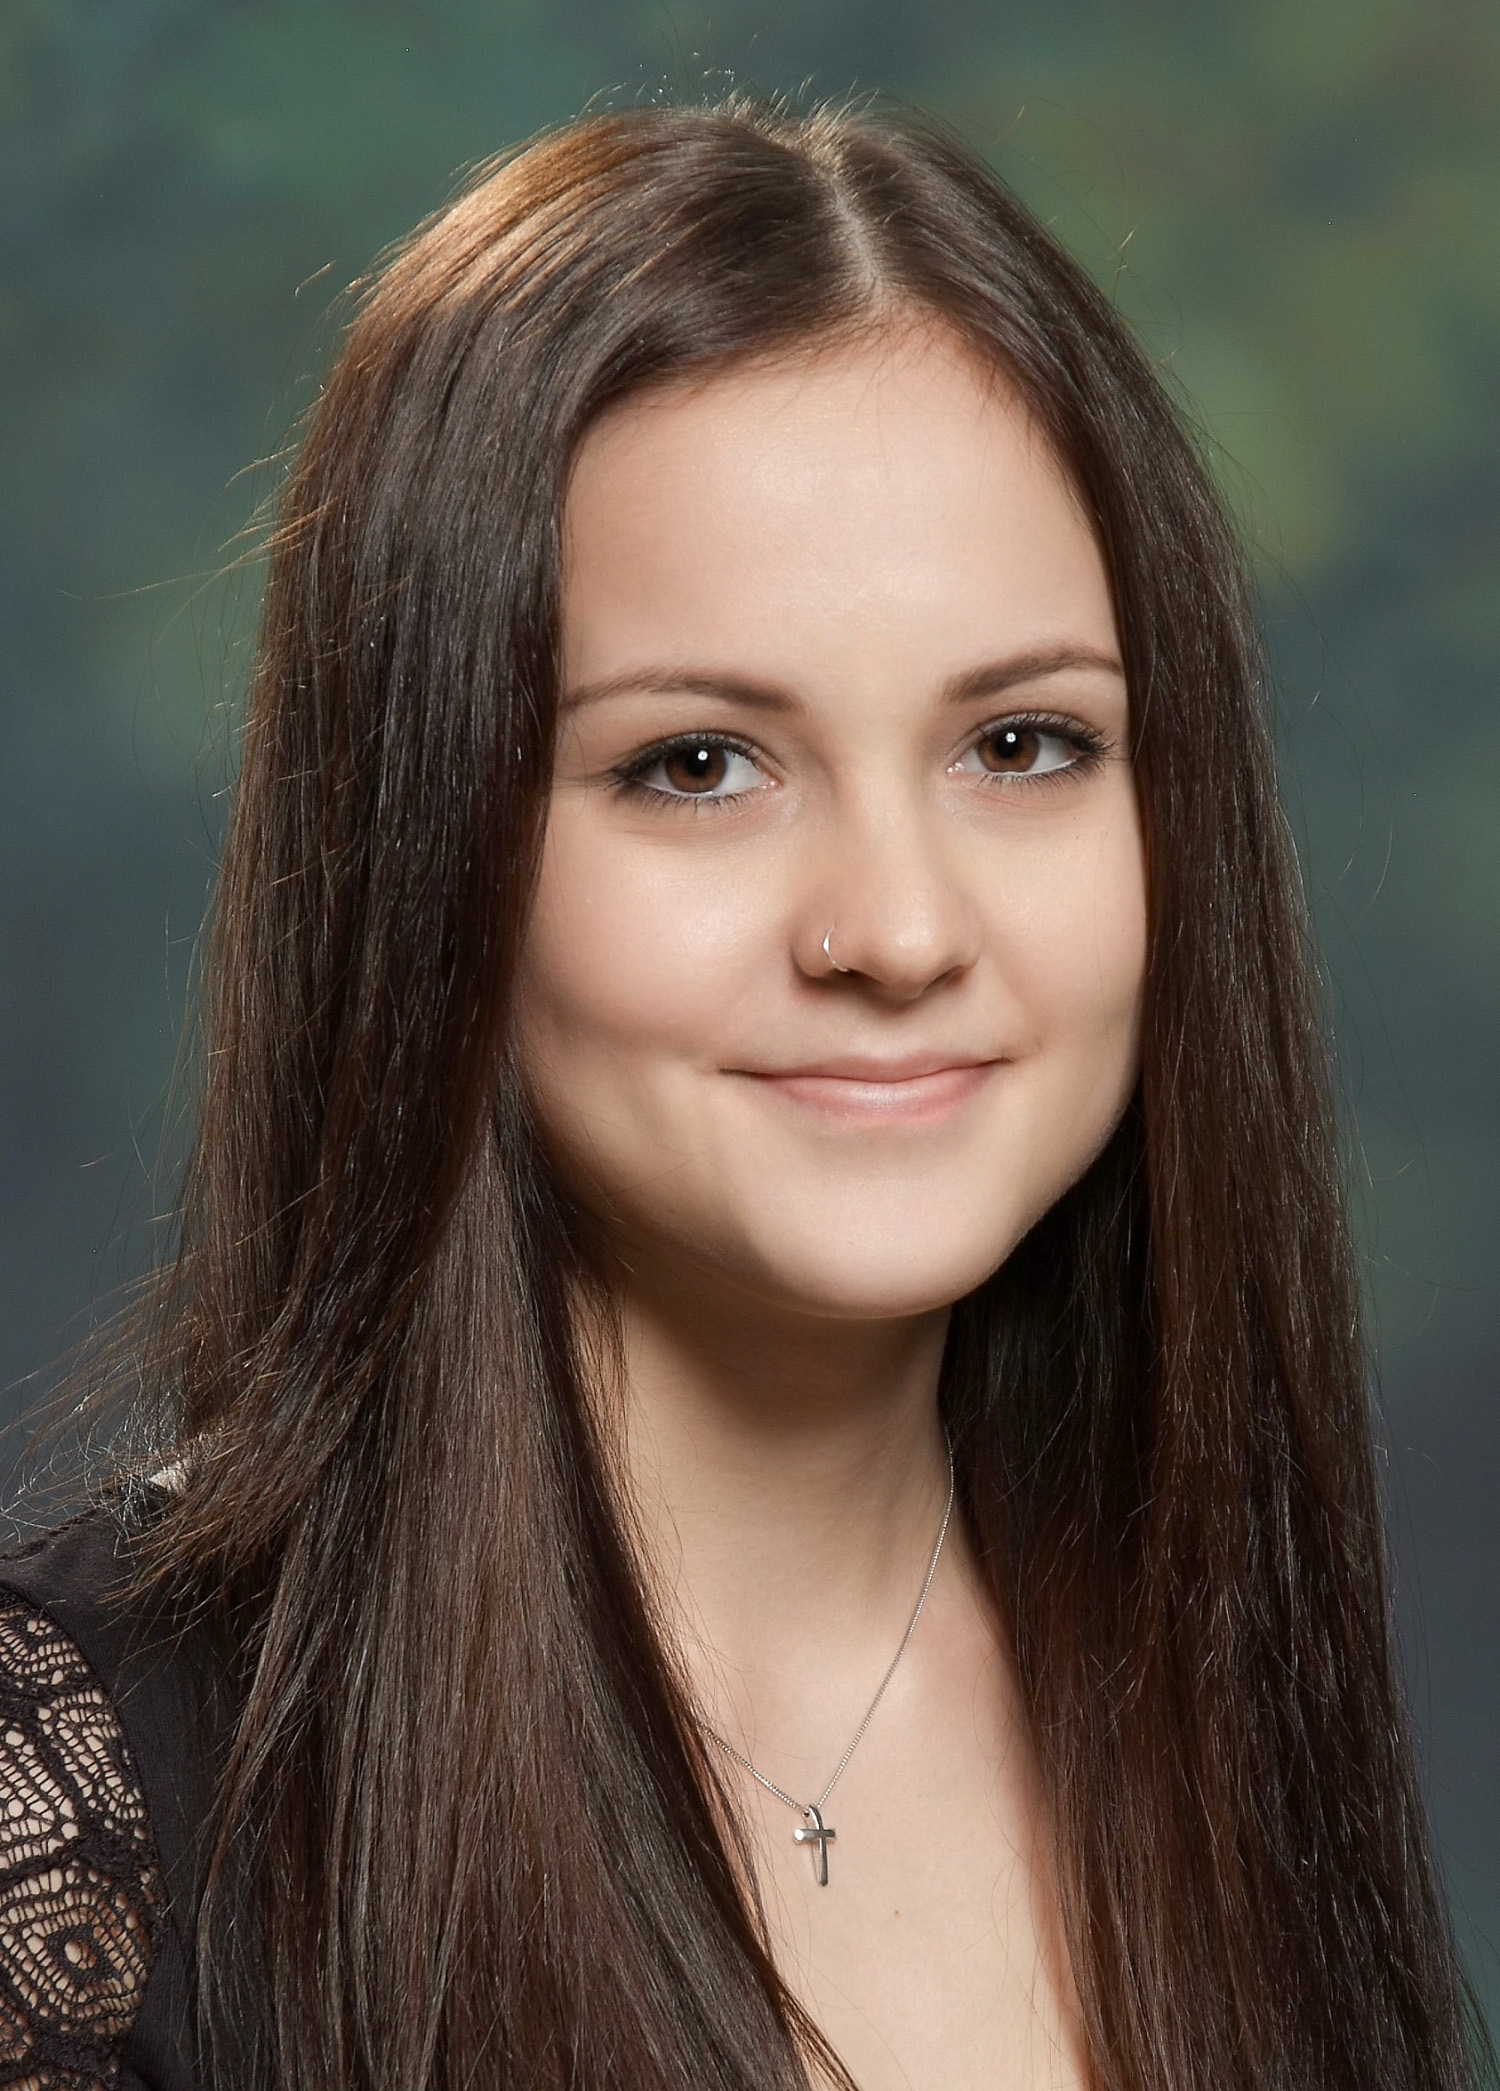
\includegraphics[height=4cm]{tiefenbrunner}
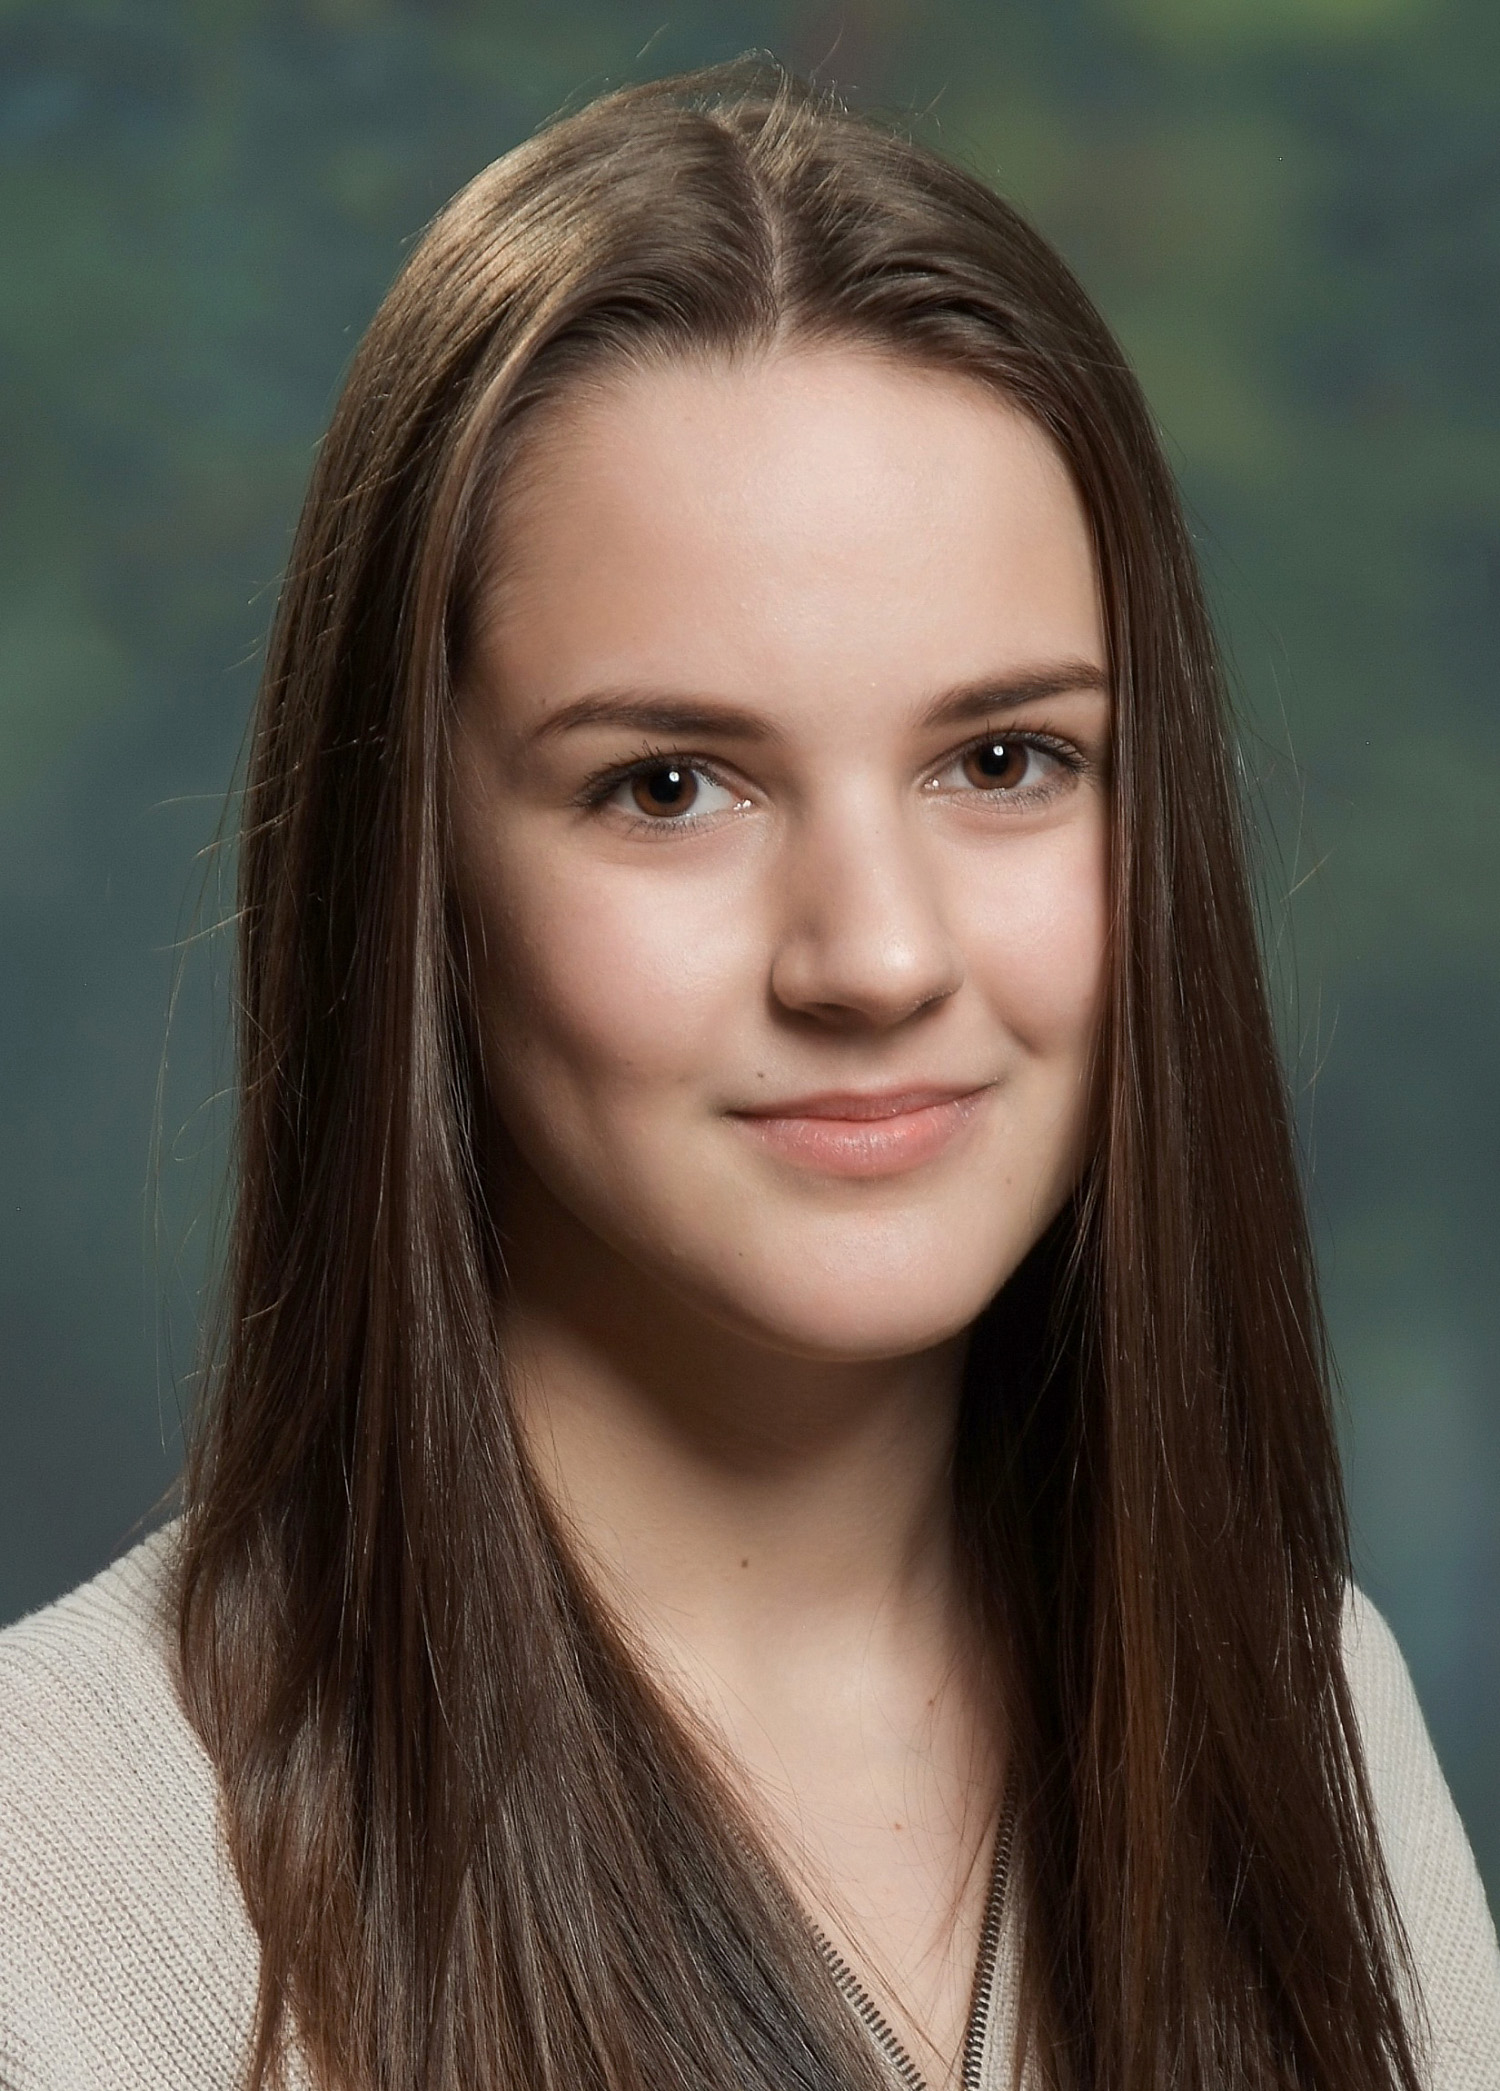
\includegraphics[height=4cm]{huber}
\subsection{Betreuer}
Neuner Dominik, MSc\\
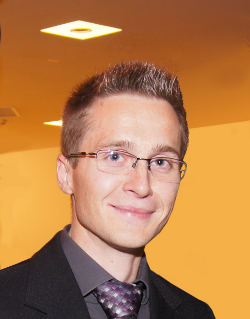
\includegraphics[height=4cm]{neuner}
\subsection{Partner}
Tourismusverband Imst\\
BHAK Imst
\subsection{Ansprechpartner}
\section{Vorerhebungen}
\subsection{Projektzieleplan}
Projektziele-Hierarchie:

Oberziel: App/Spiel GeoQuest im Appstore für jeden zum Download bereit

SMART-Prinzipien:

Spezifisch\\
Unser Ziel ist es, eine App für den Tourismusverband Imst einzurichten. Diese können Gäste nutzen um dort ganz leicht nachzusehen welche Sehenswürdigkeiten, Attraktionen und Freizeitaktivitäten die Ferienregion Imst bietet. Unser großes Ziel wird in folgende kleine Ziele eingeteilt:
\begin{itemize}
\item App programmieren, strukturieren und designen
\item Alle Sehenswürdigkeiten, Attraktionen und Freizeitmöglichkeiten sammeln und Informationen darüber herausfinden
\item Informative Texte zu jeder Sehenswürdigkeit verfassen
\item Bilder und Videos der Sehenswürdigkeiten produzieren
\end{itemize}
Messbar\\
Die App soll nicht mehr als 20000€ kosten, inklusive den Gehältern der Programmierer. Die Bilder müssen Skalierbar sein, verschwommene Bilder und Videos werden nicht genutzt. Bilder und Videos müssen schnell geladen werden. Fotoapparate, Kameras, Schnittprogramme und Photoshop dürfen 12000€ nicht überschreiten. Für Gehälter und Löhne der anderen Mitarbeiter ist ein Budget von 20000€ vorgesehen. Das geplante Budget für das Projekt sind 70000€.

Akzeptiert/Attraktiv\\
Jedes Ziel wird im Team abgesprochen, sollte jemand ein Ziel nicht akzeptieren wird diskutiert und um Verbesserungsvorschläge gebeten bis alle zufrieden sind. Das Team besteht aus einem Fotograf (zuständig für Bilder), einem Videoproduzenten (zuständig für Videos), einer Sekretärin (Texte), zwei Programmierer (App Entwicklung) und einer Webdesignerin (zuständig für CSS). 
Die App wird für Nutzer (Gäste) sehr angenehm werden, da sie einfach nachsehen können welche Sehenswürdigkeiten geöffnet (z. B. Museen) haben und was sie alles wo ansehen können.

Realistisch\\
Das gesamte Projekt geht 6 Monate. Die einzelnen Ziele gehen jedoch nicht so lange. Zuerst werden alle Sehenswürdigkeiten, Attraktionen und Freizeitmöglichkeiten angesammelt und Informationen darüber gesucht. Danach wird die App programmiert, eingerichtet, strukturiert und designt, zeitgleich werden Texte verfasst und natürlich auf die App übertragen. Zu guter Letzt werden Fotos geschossen, bearbeitet und Kurzfilme produziert.

Terminierbar
\begin{itemize}
\item Alle Sehenswürdigkeiten, Attraktionen und Freizeitmöglichkeiten sammeln und Informationen darüber herausfinden – 2 Wochen 
\item App programmieren, strukturieren und designen und Informative Texte zu jeder Sehenswürdigkeit verfassen und auf die App übertragen –  12 Wochen
\item Bilder und Videos der Sehenswürdigkeiten produzieren – 6 Wochen
\end{itemize}

\subsection{Projektumfeld}
\begin{itemize}
	
	\item Projektumfeldanalyse:
	
	Identifikation der Stakeholder:
	
	Auftraggeber: Tourismusverband Imst\\	
	Kunden\\	
	Projektbetreuer: Dominik Neuner	\\
	Mitarbeiter: Laura Huber, Julia Tiefenbrunner\\	
	Partner: BHAK Imst
	
	Charakterisierung der Stakeholder:
	
	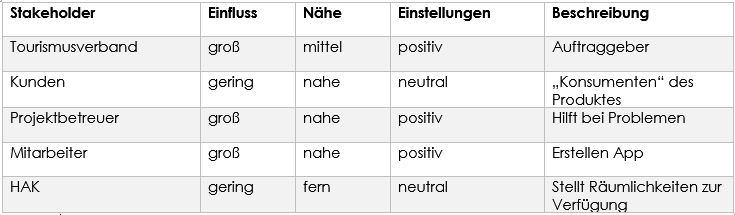
\includegraphics[height=4cm]{Stakeholder}
	
	Maßnahmen:\\
	Tourismusverband:
	\begin{itemize}
			\item Aufgabenstellung vorgeben
			\item Wünsche, Erwartungen
			\item Kontrolle des Projekts\\
	\end{itemize}
	
	Kunden:
	\begin{itemize}
	\item Feedback geben
	\item Verbesserungsvorschläge\\
	\end{itemize}
	
	Mitarbeiter:
	\begin{itemize}
		\item Erfüllung der Aufgaben
		\item Teamgeist bilden
		\item Respektvoller Umgang
		\item Zuverlässigkeit\\
	\end{itemize}
	
	HAK:
	\begin{itemize}
		\item Raumbelegung prüfen
		\item Räumlichkeiten bereitstellen\\
	\end{itemize}
	
	Grafische Darstellung des Umfeldes\\
	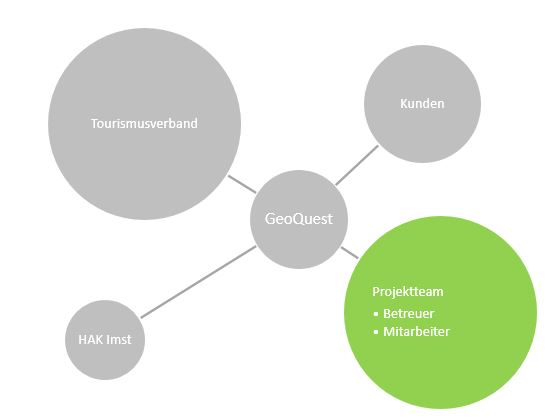
\includegraphics[height=8cm]{StakeholderGrafisch}
	
\end{itemize}
\subsection{Risikoanalyse}
\begin{itemize}
	\item Risikomatrix
	
	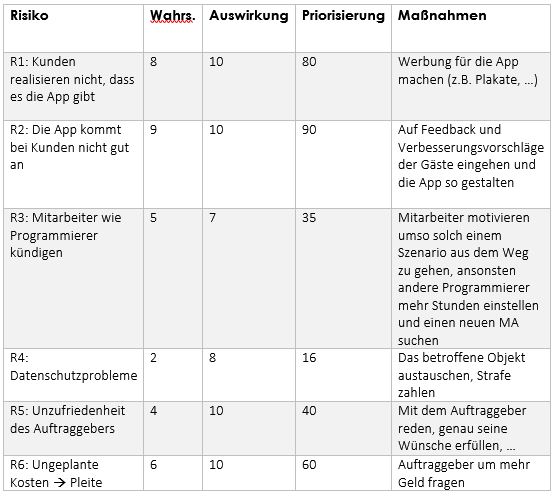
\includegraphics[height=10cm]{Risiko}\\
	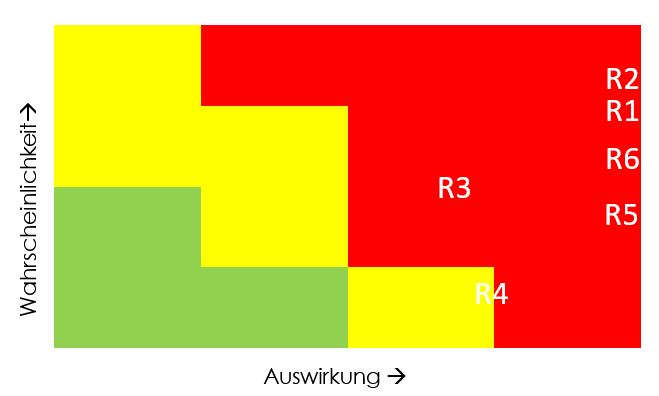
\includegraphics[height=8cm]{RMatrix}	
	
\end{itemize}
\section{Pflichtenheft}
\subsection{Zielbestimmung}
\begin{itemize}
	\item Projektbeschreibung
	\item IST-Zustand\\
	Die Stadt Imst (Tourismusverband Imst) hat eine Internetseite, (http://urlaub.imst.at/) mit Freizeitangeboten usw. Des Weiteren sind auf http://www.imst.at/de diverse Sehenswürdigkeiten unter der Registerkarte „Kultur und Brauchtum“ zu sehen.
	Eine spezielle Auflistung der Sehenswürdigkeiten, für Einheimische als auch Touristen gibt es bislang nicht, genauso wie eine „Sightseeing“-Funktion, bei der ein Programm eine Sightseeing-Tour durch Imst individuell nach Wünschen planen kann.
	Da die Stadt Imst einiges an Sehenswürdigkeiten zu bieten hat, angefangen von sämtlichen Brunnen bis zum Fasnachtshaus, bietet sich die Möglichkeit eine App für die oben genannten Funktionen zu erstellen.\\
		
	\item SOLL-Zustand\\
	Die App ermöglicht vor allem Touristen, eine individuelle Tour zu planen, und durch die übersichtliche Auflistung keine Sehenswürdigkeit zu missen.
	Neben den Sehenswürdigkeiten ist auch eine Liste für Freizeitaktivitäten und mit deren Preise und Standort vorhanden, um den Einwohnern Tirols als auch Urlaubern die Recherche über Ausflüge und Aktivitäten in Imst zu ersparen.\\
	
\end{itemize}
\subsection{Produkteinsatz und Umgebung}
\begin{itemize}
	\item Anwendungsgebiet\\
	Stadt Imst
	\item Zielgruppen\\
	Touristen und Gäste sowohl auch Einheimische
	\item Hard-/Softwareumgebung\\
	Smartphone mit entsprechender App
	
\end{itemize}
\subsection{Funktionalitäten}
\begin{itemize}
	\item MUSS-Anforderungen
	\begin{itemize}
		\item Funktional
		\item Nicht-funktional
	\end{itemize}
	\item KANN-Anforderungen
	\begin{itemize}
		\item Funktional
		\item Nicht-funktional
	\end{itemize}
\end{itemize}

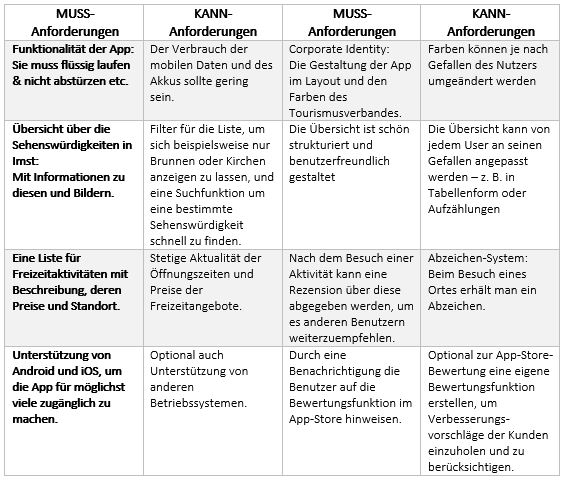
\includegraphics[height=12cm]{musskann}\\

\subsection{Testszenarien und Testfälle}
\begin{itemize}
	\item Beschreibung der Testmethodik
	\item Testfall 1
	\item Testfall 2
	\item \ldots
\end{itemize}
\subsection{Liefervereinbarung}
\begin{itemize}
	\item Lieferumfang
	\item Modus
	\item Verteilung(Deployment)
	
	Die App wird laut Terminvereinbarung im App-Store zum Download verfügbar sein.
\end{itemize}
\section{Planung}
\subsection{Projektstrukturplan}
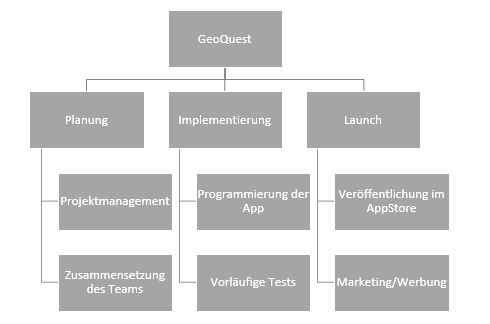
\includegraphics[height=10cm]{Projektstrukturplan}\\
\subsection{Meilensteine}
\begin{itemize}
	\item Sehenswürdigkeiten und zugehörige Fragen finden
	\item Datenbank anlegen
	\item Tabellen für Datenbank anlegen
	\item UML-Diagramm erstellen
	\item Grundstruktur programmieren
	\item Datenbank befüllen
	\item Backend-Benutzer programmieren
	\item PHP-Klasse für Datenbankverbindung
	\item Interface für Benutzer mit Methoden
	\item Benutzer-Klasse programmieren
	\item Interface für Fragen mit Methoden
	\item Fragen-Klasse programmieren
	\item Tabellen verbinden
	\item Testphase
	\item Launch im App-Store
\end{itemize}
\subsection{Gant-Chart}
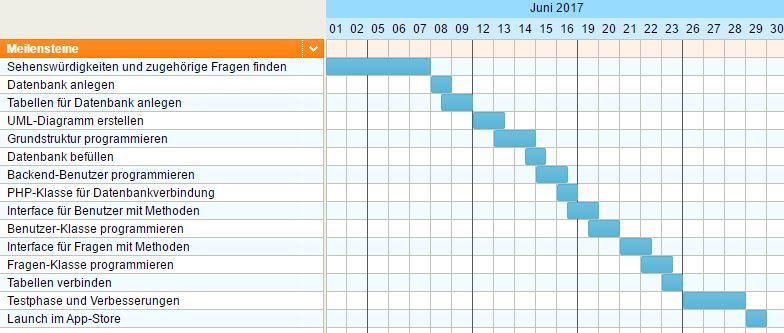
\includegraphics[width=15cm]{meilensteine}\\
\subsection{Abnahmekriterien}
\subsection{Pläne zur Evaluierung}
\subsection{Ergänzungen und zu klärende Punkte}

\chapter{Vorstellung des Produktes}
Vorstellung des fertigen Produktes anhand von Screenshots, Bildern, Erklärungen.

\chapter{Eingesetzte Technologien}
\begin{itemize}
	\item Kurzbeschreibung aller Technologien, die verwendet wurden.
	\item Technologien die aus dem Unterricht bekannt sind, nur nennen und deren  Einsatzzweck im Projekt beschreiben, nicht die Technologien selbst.
	\item Technologien die aus dem Unterricht nicht bekannt sind, im Detail beschreiben incl. deren Einsatz im Projekt
	\item Fokus aus eingesetzten Frameworks
	
	
	Technologien:
	\begin{itemize}
	\item HTML – für Strukturierung und Zuweisung der Texte auf den verschiedenen Seiten der App.
	\item CSS – für das Layout der App.
	\item JavaScript – Programmierung der verschiedenen Funktionen wie Buttons, Analysierung der Sehenswürdigkeiten (mit zum Beispiel QR-Code-Scanner) und laden der Texte und Bilder dazu, usw.\\
	\end{itemize}

	Programme:
	\begin{itemize}
	\item PHP Storm\\\\\\
	\end{itemize}
	
	Unsere mobile Web-App basiert auf dem Programm PHP-Storm, dort setzen wir die oben genannten und erklärten Technologien HTML, CSS und JavaScript ein. Als Framework benützen wir das kostenlose LungoJS 1.2, das im folgenden Absatz genauer beschrieben wird:
	Funktionsumfang: Entwicklung mobiler Web-Apps mit Unterstützung für Touch-Gesten, WebSQL, Browserverlauf, Geolocation, und vielem mehr.
	Es handelt sich um ein mobiles Framework zur Entwicklung HTML5- basierter Apps für iOS, Android, Blackberry und Windows Phone 7. LungoJS erzeugt semantisches Mark-up und versteht sich auf die Auswertung von Touch- Ereignissen wie Wischbewegungen, die dynamische Handhabung des Ausrichtungswechsels des Displays, WebSQL, und Geolocation. Außerdem können Sie damit den Browserverlauf in Ihren Apps nutzen.
	Alle UI-Elemente sind vektorbasiert, so dass die Darstellungsqualität unabhängig von der Auflösungsdichte des Displays gewährleistet ist. Das Framework lässt sich mit Hilfe der so genannten Sugars erweitern. Die resultierenden Apps können Sie sowohl über Ihre eigene Website als auch über die offiziellen Distributionskanäle vertreiben.
	
\end{itemize}
\chapter{Problemanalyse}
\section{USE-Case-Analyse}
\begin{itemize}
	\item UseCases auf Basis von Benutzerzielen identifizieren: 
	\begin{itemize}
		\item Benutzer eines Systems identifizieren
		\item Benutzerziele identifizieren (Interviews)
		\item Use-Case-Liste pro Benutzer definieren
	\end{itemize}
	\item UseCases auf Basis von Ereignissen identifizieren: 
	\begin{itemize}
		\item Externes Event triggert einen Prozess
		\item zeitliches Event triggert einen Prozess (Zeitpunkt wird erreicht) 
		\item State-Event (Zustandsänderung im System triggert einen Prozess)
	\end{itemize}
	\item Werkzeuge:
	\begin{itemize}
		\item USE-Case-Beschreibungen (textuell, tabellarisch)
		\item USE-Case-Diagramm
		\item Aktivitätsdiagramm für den Use-Case (Interaktion zwischen Akteur und System abbilden)
		\item System-Sequenzdiagramm (Spezialfall eines Sequenzdiagramms: Nur 1 Akteur und 1 Objekt, das Objekt ist das komplette System, es geht um die Input/Output Requirements, die abzubilden sind)
	\end{itemize}
\end{itemize}
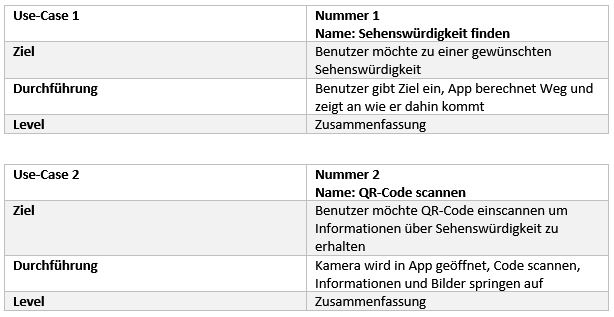
\includegraphics[width=15cm]{usecasetabelle}\\\\\\
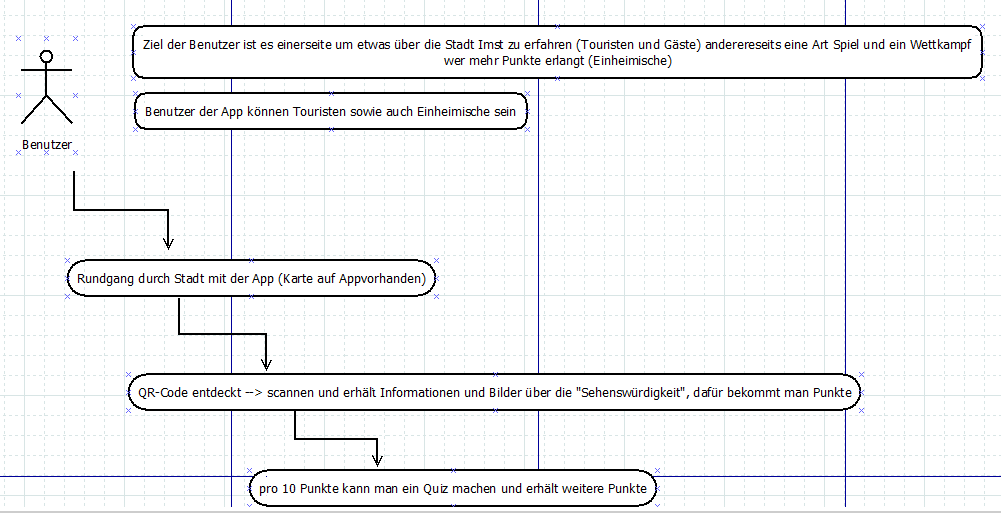
\includegraphics[height=8cm]{usecase}

\section{Domain-Class-Modelling}
\begin{itemize}
	\item "Dinge" (Rollen, Einheiten, Geräte, Events etc.) identifizieren, um die es im Projekt geht
	\item ER-Modellierung oder Klassendiagramme
	\item Zustandsdiagramme (zur Darstellung des Lebenszyklus von Domain-Klassen darstellen)
\end{itemize}

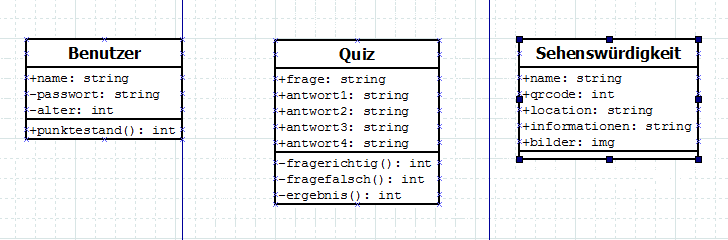
\includegraphics[height=5cm]{domainclass}

\section{User-Interface-Design}
\begin{itemize}
	\item Mockup\\
	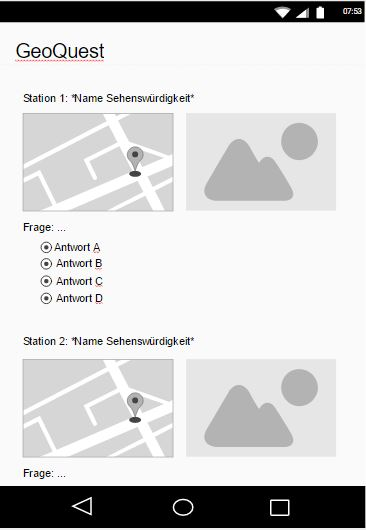
\includegraphics[width=10cm]{mockup}\\
	
\end{itemize}


\chapter{Systementwurf}

\section{Architektur}

\subsection{Design der Komponenten}

Darstellung und Beschreibung der Systemarchitektur;

\begin{itemize}
	\item  statische Zerlegung des Systems in seine physischen Bestandteile (Komponenten, Komponentendiagramm)
	\item (textuelle) Beschreibung des dynamischen Zusammenwirkens aller Komponenten 
	\item (textuelle) Beschreibung der Strategie für die Architektur, d. h. wie die Architektur in Statik und Dynamik funktionieren soll.
	\item Verwendung von Referenzarchitekturen bzw. Architekturmustern (als Schablonen, z.B. MVC. Plugin, Pipes and Filters)
	\begin{itemize}
		\item MVC
		\item Schichten
		\item Pipes
		\item Request Broker
		\item Service-Oriented
	\end{itemize}
\end{itemize}

\subsection{Benutzerschnittstellen} 
\begin{itemize}
	\item Design des UIs
	\item Dialoge, Dialogsteuerung, Ergonomie, Gestaltung, Eingabeüberprüfungen
\end{itemize}

\subsection{Datenhaltunskonzept}
\begin{itemize}
	\item Design der Datenbank (ER-Modell)
	\item Design des Zugriffs auf diese Daten (Datenhaltungskonzept)
	\item Caching, Transaktionen
\end{itemize}

\subsection{Konzept für Ausnahmebehandlung}
\begin{itemize}
	\item Systemweite Festlegung, wie mit Exceptions umgegangen wird
	\item Exceptions sind primär aus den Bereichen UI, Persistenz, Workflow-Management
\end{itemize}

\subsection{Sicherheitskonzept}
Beschreibung aller sicherheitsrelevanten Designentscheidungen

\begin{itemize}
	\item Design der Security-Elemente
	\item Design von Safety-Elementen (Fehlertoleranz, Verfügbarkeit etc.)
\end{itemize}

\subsection{Design der Testumgebung}
\begin{itemize}
	\item wie wird getestet (Unit-Testing, Integrationstesting, Systemtests, Akzeptanztests)
	\item Testumgebung, Testprozess, Teststrategie, Testmethoden, Testfälle
\end{itemize}


\subsection{Desing der Ausführungsumgebung}
\begin{itemize}
	\item Deployment (DevOps)
	\item Betrieb (besonders Hoch- und Hertunerfahren der Anwendung)
\end{itemize}

\section{Detailentwurf}

Design jedes einzelnen USE-Cases

\begin{itemize}
	\item Design-Klassendiagramme vom Domain-Klassendiagramm ableiten (incl. detaillierter Darstellung und Verwendung von Vererbungshierarchichen, abstrakten Klassen, Interfaces)
	\item Sequenzdiagramme vom System-Sequenz-Diagramm ableiten
	\item Aktivitätsdiagramme
	\item Detaillierte Zustandsdiagramme für wichtige Klassen
\end{itemize}

Verwendung von CRC-Cards (Class, Responsibilities, Collaboration) für die Klassen
\begin{itemize}
	\item um Verantwortlichkeiten und Zusammenarbeit zwischen Klassen zu definieren und
	\item um auf den Entwurf der Geschäftslogik zu fokussieren
\end{itemize}

Design-Klassen für jeden einzelnen USE-Case können z.B. sein:

\begin{itemize}
	\item UI-Klassen
	\item Data-Access-Klassen
	\item Entity-Klassen (Domain-Klassen)
	\item Controller-Klassen
	\item Business-Logik-Klassen
	\item View-Klassen
\end{itemize}

Optimierung des Entwurfs (Modularisierung, Erweiterbarkeit, Lesbarkeit):

\begin{itemize}
	\item Kopplung optimieren
	\item Kohäsion optimieren
	\item SOLID
	\item Entwurfsmuster einsetzen
\end{itemize}

\chapter{Implementierung}
Detaillierte Beschreibung der Implementierung aller Teilkomponenten der Software entlang der zentralsten Use-Cases:

\begin{itemize}
	\item GUI-Implementierung
	\item Controllerlogik
	\item Geschäftslogik
	\item Datenbankzugriffe
\end{itemize}

Detaillierte Beschreibung der Teststrategie (Testdriven Development):

\begin{itemize}
	\item UNIT-Tests (Funktional)
	\item Integrationstests
\end{itemize}

Zu Codesequenzen:
\begin{itemize}
	\item kurze Codesequenzen direkt im Text (mit Zeilnnummern auf die man in der Beschreibung verweisen kann)
	\item lange Codesequenzen in den Anhang (mit Zeilennummer) und darauf verweisen (wie z.B. hier \cref{qj})
\end{itemize}

\chapter{Deployment}
\begin{itemize}
	\item Umsetzung der Ausführungsumgebung
	\item Deployment
	\item DevOps-Thema
\end{itemize}

\chapter{Tests}

\section{Systemtests} 
Systemtests aller implementierten Funktionalitäten lt. Pflichtenheft
\begin{itemize}
	\item Beschreibung der Teststrategie
	\item Testfall 1
	\item Testfall 2
	\item Tesfall 3
	\item …
\end{itemize}

\section{Akzeptanztests}

\chapter{Projektevaluation}
siehe Projektmanagement-Unterricht

\chapter{Benutzerhandbuch} 
falls im Projekt gefordert

\chapter{Betriebswirtschaftlicher Kontext}
BW-Teil

\chapter{Zusammenfassung}
\begin{itemize}
	\item Etwas längere Form des Abstracts
	\item Detaillierte Beschreibung des Outputs der Arbeit
\end{itemize}